%!TEX root = thesis.tex

\chapter{Visualisation Design}
\label{chap:visualisation-design}

Following the exploratory field study (see Chapter~\ref{chap:exploratory-field-study}), a strategy for visualisation prototyping and evaluation was developed. This strategy was based on the analysis of the literature and the evaluation of the results of the exploratory field study. A collaborative approach was taken, working with a live coder to integrate visuals into the live coding process. The rationale behind developing visualisations, the approach taken to develop the visualisations and the resulting visualisations are discussed within this chapter.

\section{Rationale}

% {\color{red}\cite{Ware2013a,McLean2010a,Purchase1996} will be useful here.}

The exploratory field study established and examined questions regarding the projection of source code during live coding performances including: ``Is source code the best method of communicating the performance?'' and ``Are there alternative methods?''. Results suggested that there was potential for visualisation of the live coding process and identified understanding and enjoyment as valid measures of the audience.

Evaluation of the literature had identified the need for visualisations that helped live coding audiences understand and enjoy the live coding performance. To this end, two sets of visualisations were developed. The first was intended to increase the enjoyment of the audience, enhancing aesthetic appeal and was labelled the ``aesthetic condition''. The second was intended to communicate the live coding process, help the audience to understand the programmatic aspects of the performance and was labelled the ``didactic condition''.

\section{Requirements}

In order to systematically and efficiently develop a visualisation design strategy, two stakeholders were identified. These included the live coder and the intended audience.

Evaluation of the visualisation prototype required application to a live coding performance. To achieve this, the live coder would need to apply the visualisations to a live performance. To this end, discussions with the live coder identified functional requirements including simultaneous display of source code and visualisations and visualisations depicting the progression of the performance accurately. Non-functional requirements identified included performance, as the nature of live coding is realtime, and reliability, as a single failure in the visualisations could cause catastrophic failure within the live coding performance.

Typical live coding performances consist of around four instruments. This is to maintain musical consistency throughout the performance but to also allow for musical progression. It was identified that to accurately visualise a live coding performance, the visuals would also need to have similar progression while also maintaining consistency throughout the performance using a visual palette of colours, shapes and animations.

The intended audience was identified as a critical stakeholder in the ultimate effectiveness of the visualisations developed. The audience evaluated in the initial field study provided the basis for these requirements.

% The source code caused fatigue, however to understand the program, seeing the whole development process (all the code) was necessary.

Requirements identified by the audience during the intial field study indicated that \more
% -discuss audience requirements identified from first study

Fundamental to live coding is the performance element. Live coding requires a reliable programming environment. Visualisations developed for this environment required that the chance of failure were minimised. To mitigate the chance of a failure in the live coding environment, a test strategy was developed for the visualisations to ensure that they did not cause unrecoverable failures and did not cause memory leaks.

% Timeline constraints were also identified as a potential risk factor in the development and evaluation of the visualisations. Mitigation involved developing a flexible, iteration based development plan with estimated milestones.

-ensure that the visualisations would provide a benefit and would not negatively impact the performance... mitigated by the iteration based approach to developing the visualisations

-ensure that the visualisations would not interfere with the live coder... \more

\section{Design}

\begin{figure}
  \centering 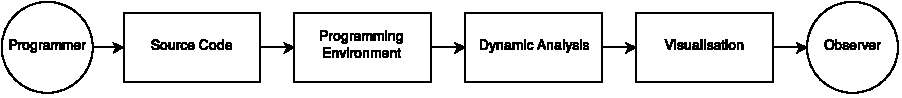
\includegraphics[width=\columnwidth]{../images/diagrams/knowledge-flow-initial.pdf}
  \caption{Knowledge flow from programmer to observer as directed by the visualisation technique employed.}
\label{fig:knowledge-flow-initial}
\end{figure}

The intial iteration of the visualisation prototype consisted of two separate conditions. Each condition consisted of four visual progressions with the intention of representing the addition and removal of instruments during the live coding performance. Visualisations employed dynamic analysis of the running program to generate the visuals. The model of knowledge flow from programmer to observer is shown in Figure~\ref{fig:knowledge-flow-initial}.

The first visualisation condition was labelled the ``aesthetic'' condition reflecting the intention to improve enjoyment during the live coding performance. The second visualisation condition was labelled the ``didactic'' condition with an intended goal of improving understanding during the live coding performance.

% The design of the initial visualisations focussed on the application of the literature on visualisation design to the field of software visualisation and the application to the visualisation of live code.

-music visualisation is an extremely rich and open-ended task, so to guide the development of the visualisations for our lab study... \more

-guidelines set out by mclean were used in understanding the application of visualisation to live coding...
\cite{McLean2010a}... \more

-guidelines set out by ware were used in developing the visualisations...
% - what are the guidelines used
\cite{Ware2013a}... \more

Geometrics used included... \more

Colour schemes, although varying slightly throughout the visualisations, consisted of a colour palette of red, orange and blue with red and orange used heavily throughout the visualisations and blue used for emphasis and visual interest.

Animations were used when... \more

\subsection{Didactic Visualisation}
\label{sec:didactic-visualisation}

\begin{figure}
\centering
\begin{subfigure}{.5\textwidth}
  \centering
  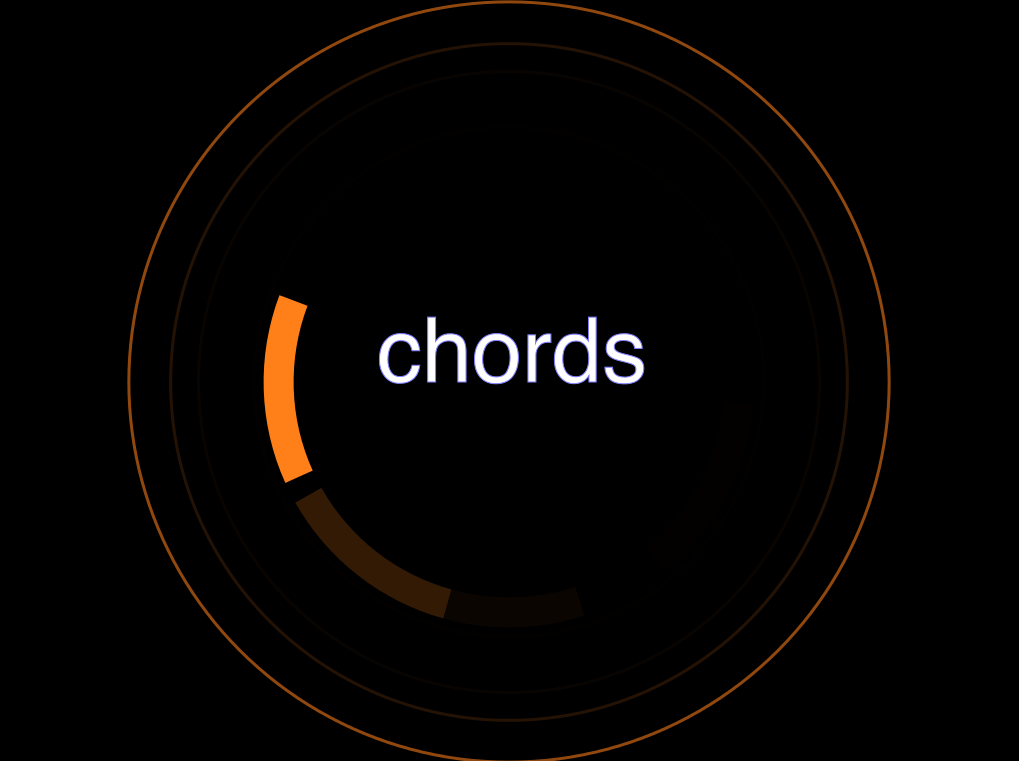
\includegraphics[width=.95\linewidth]{../study-2/results/visualisations/didactic-one.png}
  \caption{Phase 1}
  \label{fig:didactic-one}
\end{subfigure}%
\begin{subfigure}{.5\textwidth}
  \centering
  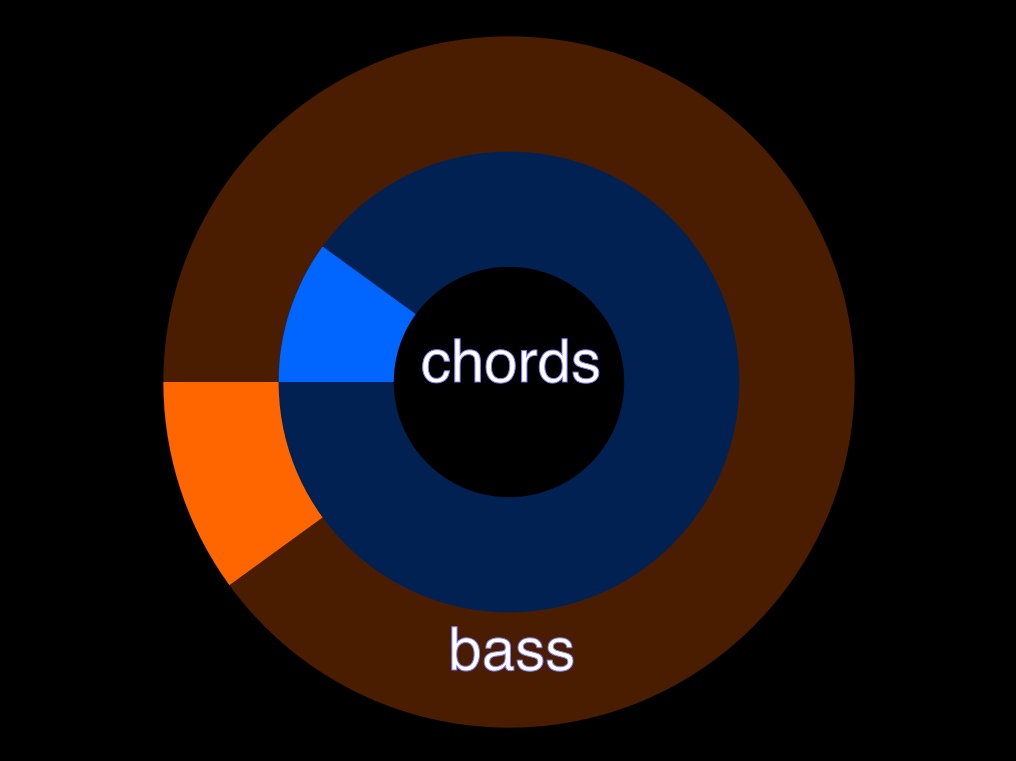
\includegraphics[width=.95\linewidth]{../study-2/results/visualisations/didactic-two.png}
  \caption{Phase 2}
  \label{fig:didactic-two}
\end{subfigure}\\
\begin{subfigure}{.5\textwidth}
  \centering
  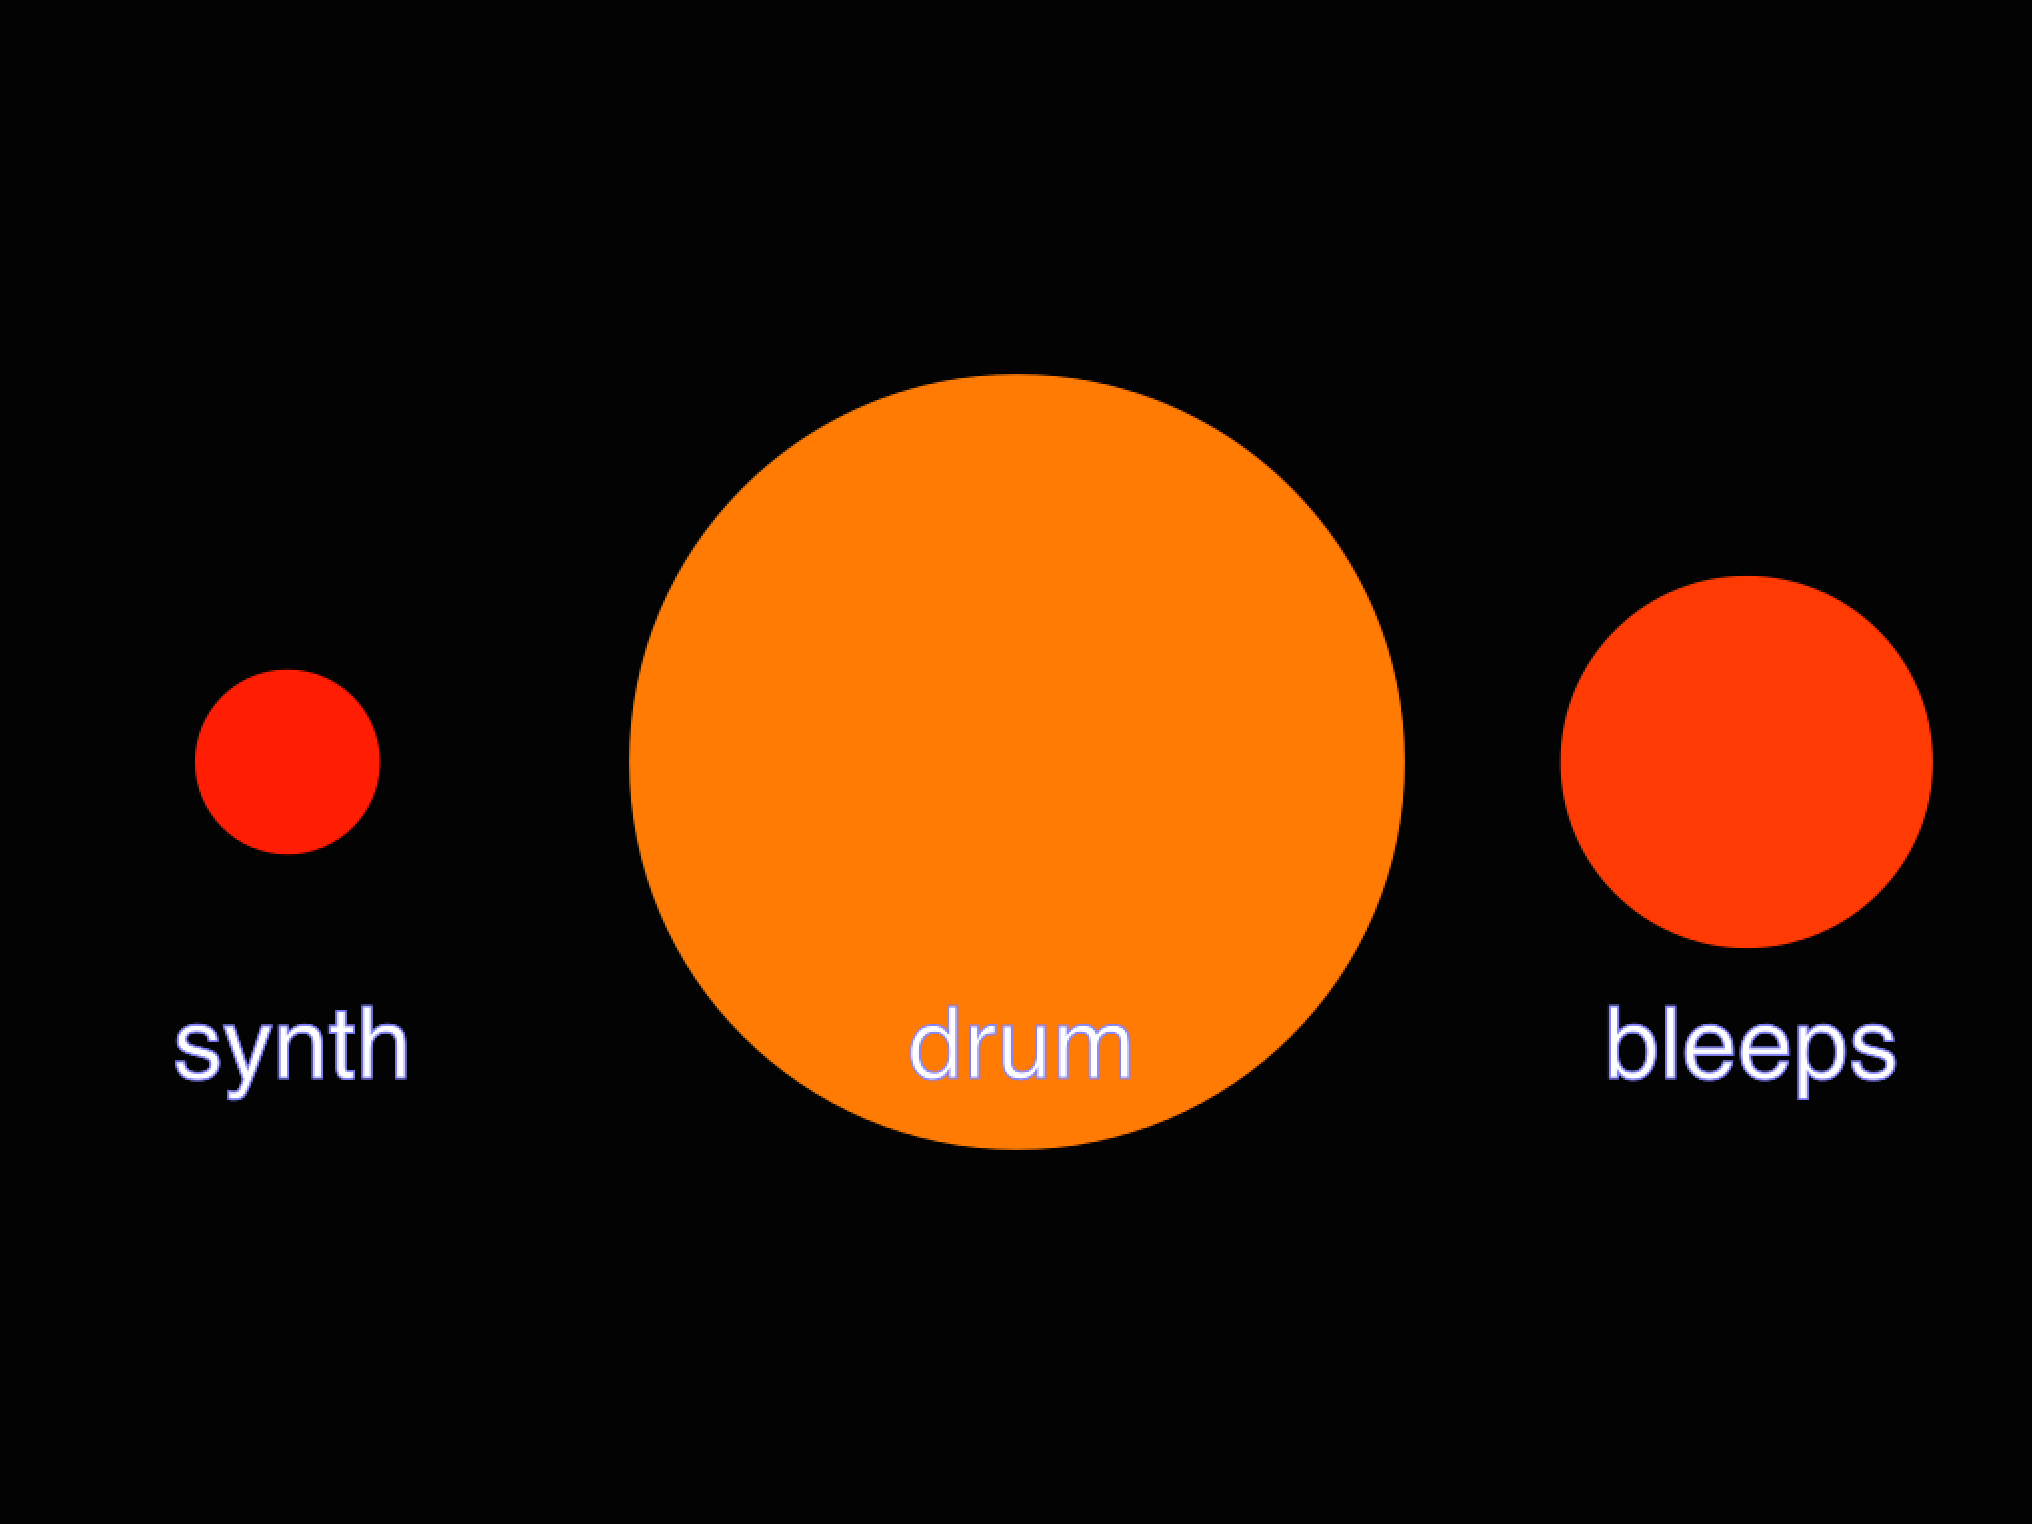
\includegraphics[width=.95\linewidth]{../study-2/results/visualisations/didactic-three.png}
  \caption{Phase 3}
  \label{fig:didactic-three}
\end{subfigure}%
\begin{subfigure}{.5\textwidth}
  \centering
  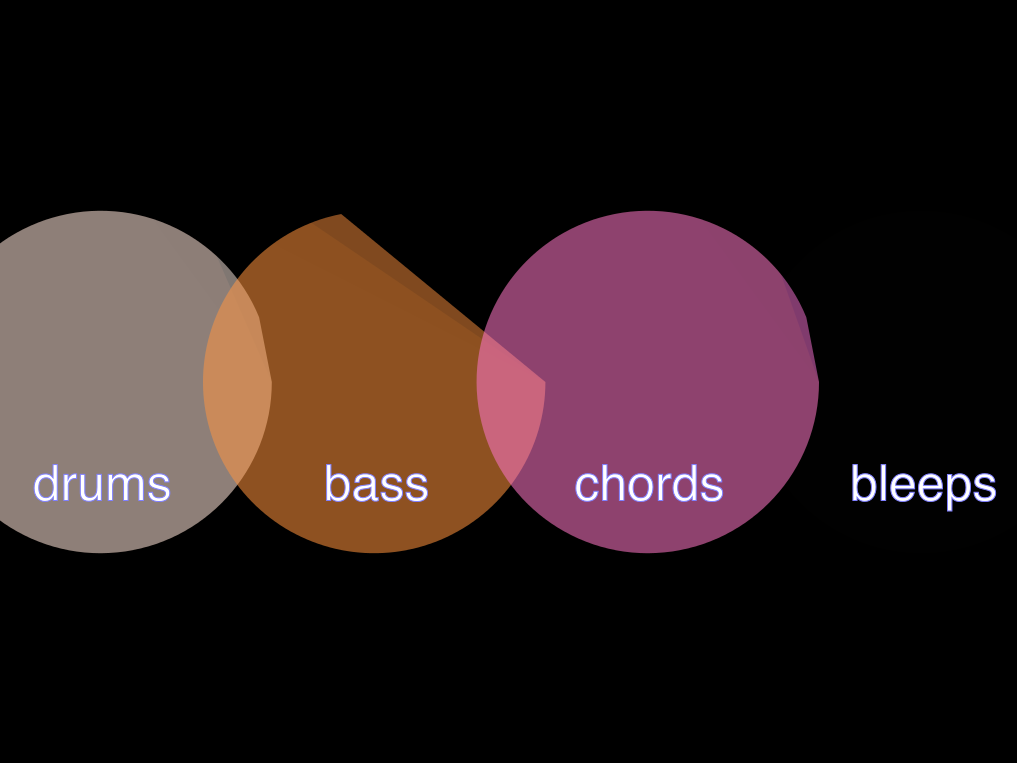
\includegraphics[width=.95\linewidth]{../study-2/results/visualisations/didactic-four.png}
  \caption{Phase 4}
  \label{fig:didactic-four}
\end{subfigure}

\caption[Didactic visualisation phases]{The four phases of the didactic visualisation.}
\label{fig:didactic-visualisations}
\end{figure}


The didactic visualisation (shown in Figure~\ref{fig:didactic-visualisations}) attempted to communicate \emph{information} about the actions of the programmer, prominently displaying the \emph{names} of the active (source code) functions and the ``time until next execution'' for each function. This ``time until next execution'' known as the ``callback rate'' was a primary feature of the programming environment and an essential part of musical live coding. Bright colours and solid shapes were used to ensure constant visibility and to communicate the intention of the underlying code. 

The stages of this visualisation attempted to address the issues indicated during the exploratory field study. These included the lack of an overview of the source code and program behaviour, the difficulty in linking changes to the source code and the flicking between source code screens. The didactic visualisations proceeded through four stages, with progression made depending on the number of active functions (instruments).

Phase one, as shown in Figure~\ref{fig:didactic-one}, displayed the name of the one active function in the centre of the screen. Two other major visual elements were present including a short circular line segment rotating and a pulsing circle. Both visual elements were mapped to the callback rate of the active function. Phase two, as shown in Figure~\ref{fig:didactic-two}, displayed the name of two active functions. Two ring-shaped visual elements represented the two functions. Each ring-shape was divided into ten segments with each segment coloured according to the callback progress of the active functions. Phase three, as shown in Figure~\ref{fig:didactic-three}, displayed three active functions as pulsing circles according to the progress of the active function callbacks. Finally, phase four, as shown in Figure~\ref{fig:didactic-four}, displayed four active functions as circles with a colour fill according to the progress of the active function callbacks.

\subsection{Aesthetic Visualisation}
\label{sec:aesthetic-visualisation}

\begin{figure}
\centering
\begin{subfigure}{.5\textwidth}
  \centering
  
\includegraphics[width=.95\linewidth]{../study-2/results/visualisations/aesthetic-one.png}
  \caption{Phase 1}
  \label{fig:aesthetic-one}
\end{subfigure}%
\begin{subfigure}{.5\textwidth}
  \centering
  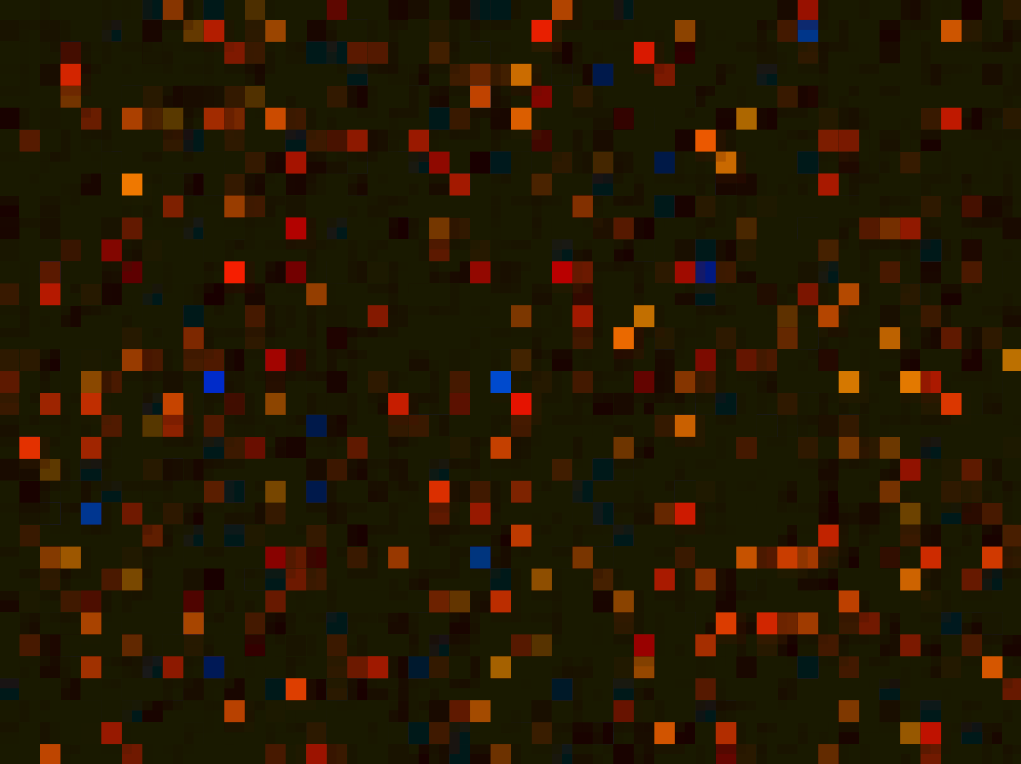
\includegraphics[width=.95\linewidth]{../study-2/results/visualisations/aesthetic-two.png}
  \caption{Phase 2}
  \label{fig:aesthetic-two}
\end{subfigure}\\
\begin{subfigure}{.5\textwidth}
  \centering
  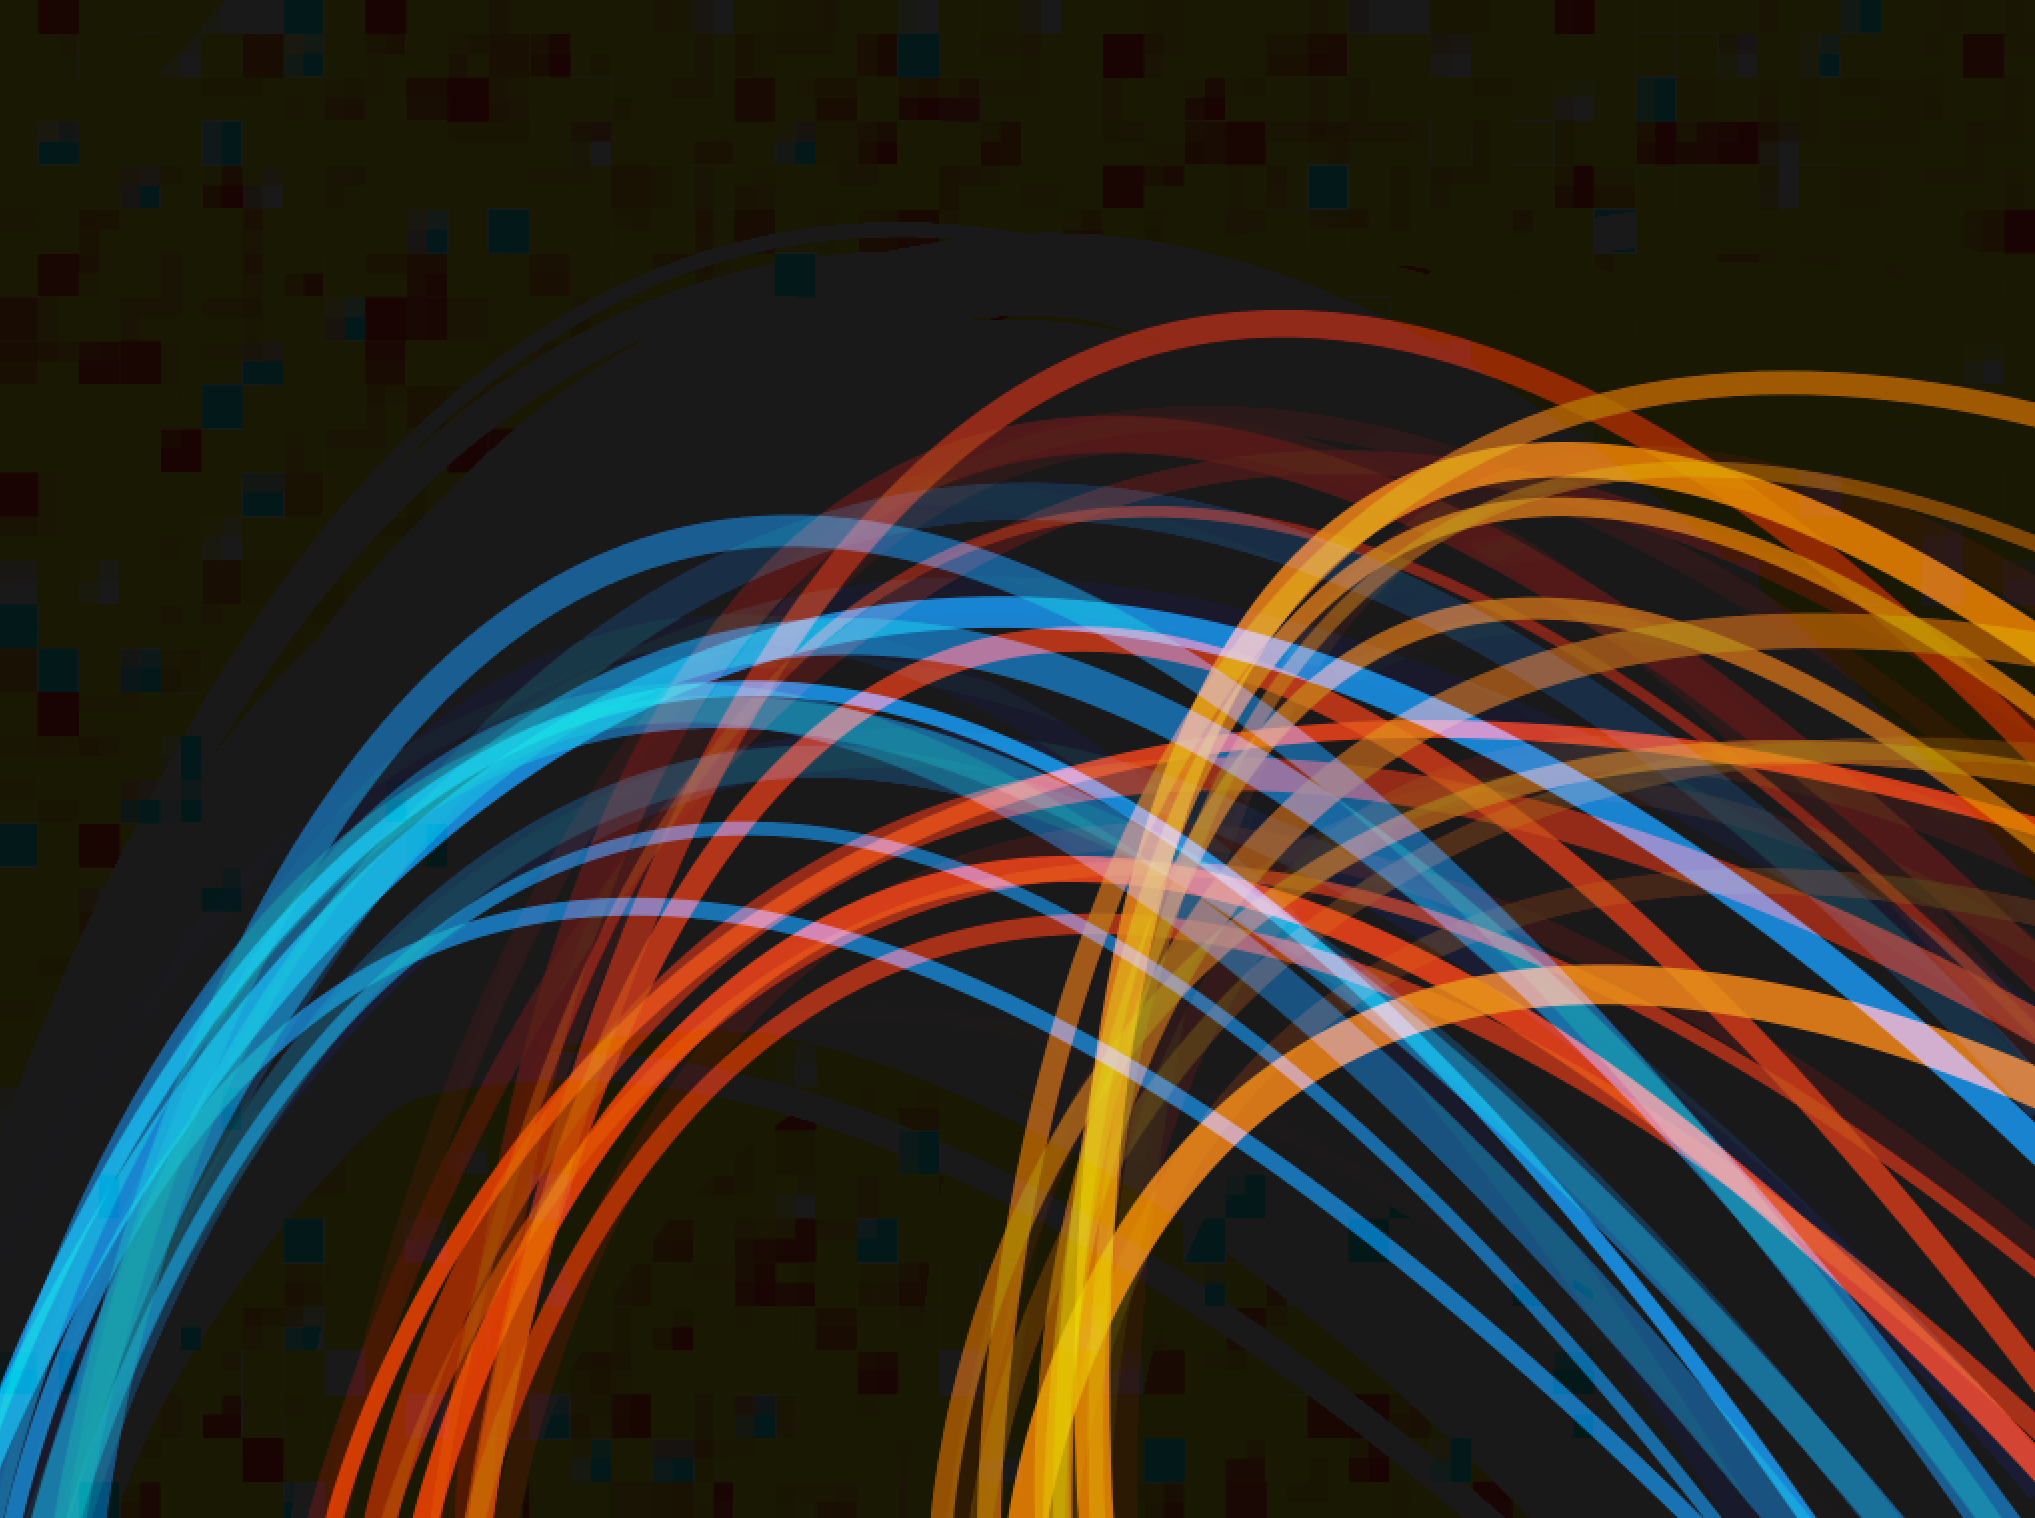
\includegraphics[width=.95\linewidth]{../study-2/results/visualisations/aesthetic-three.png}
  \caption{Phase 3}
  \label{fig:aesthetic-three}
\end{subfigure}%
\begin{subfigure}{.5\textwidth}
  \centering
  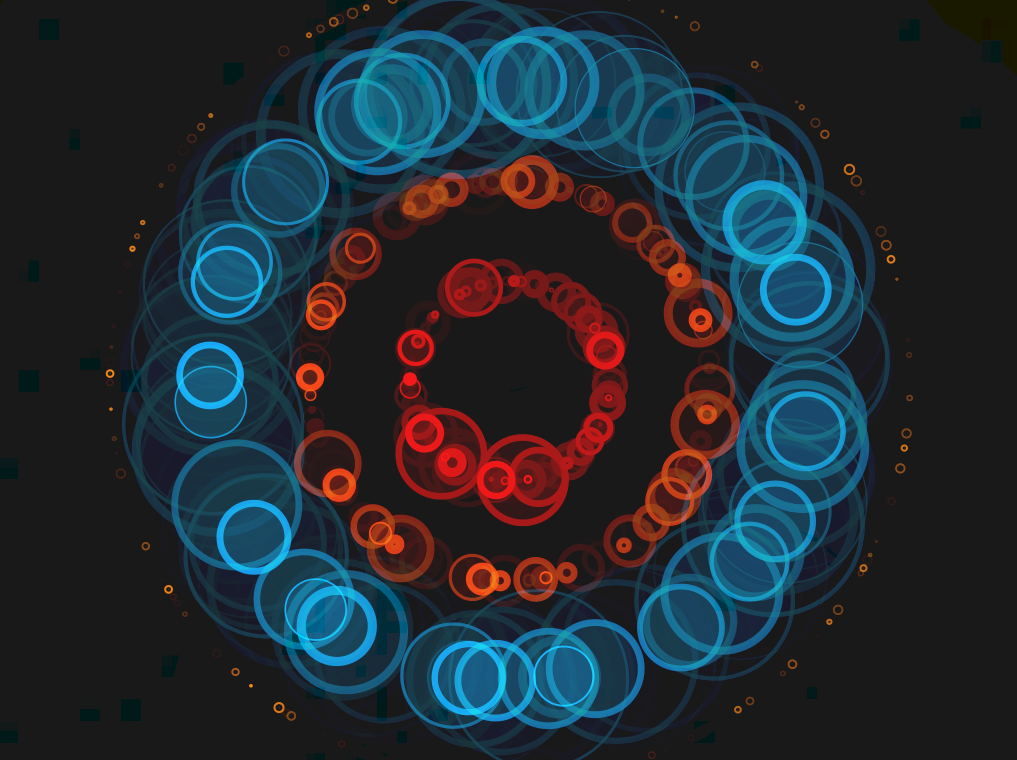
\includegraphics[width=.95\linewidth]{../study-2/results/visualisations/aesthetic-four.png}
  \caption{Phase 4}
  \label{fig:aesthetic-four}
\end{subfigure}

\caption[Aesthetic visualisation phases]{The four phases of the aesthetic visualisation.}
\label{fig:aesthetic-visualisations}
\end{figure}

The aesthetic visualisation technique was designed to react to the programmer's activity in a more abstract way, to maximise aesthetic appeal~\cite{Cawthon2007} and to engage the audience's interest. Although still based on the source code and the livecoder's edits, the generation of shapes was driven by instrument volume and synchronised with the musical beat. These were secondary features of the programming language and features resulting from the output of the running program as opposed to the callback rate, a primary feature, used in the didactic visualisations.

The emphasis for the aesthetic visualisation was on the artistic appeal of the visuals (see Figure~\ref{fig:aesthetic-visualisations}), including more variety in visual structure and colour. As in the didactic condition, the aesthetic visualisations proceeded through four stages, based on the number of active functions (instruments), but these visuals had no textual labels and they moved and interacted with each other over the entire projected scene.



Phase one, as shown in Figure~\ref{fig:aesthetic-one}, ...

Phase two, as shown in Figure~\ref{fig:aesthetic-two}...

Phase three, as shown in Figure~\ref{fig:aesthetic-three}...

Phase four, as shown in Figure~\ref{fig:aesthetic-four}...

\section{Development}

Collaboration with a live coder was required to ensure the visualisations integrated with the live coding performance workflow and progression.

Cairo was used as the supporting graphics library for visualisations implementation with the final prototype consisting of 1000 \ac{SLOC}. Visualisations were written in pure xtlang, as part of the Extempore live coding environment.

% what other considerations had to be made during development?

\section{Summary}

Evaluation of the visualisation technique was required 
-needed to test out the assumptions made while designing the visualisation prototype
-wanted to compare the two visualisation techniques
-compare the two techniques and build on this for future iterations



